\chapter{Wybrane narzędzia i technologie}


W pracy magisterskiej podczas opracowywania i wdrażania systemu wykorzystano rozmaite narzędzia i technologie. Każde narzędzie odgrywa kluczową rolę w zapewnieniu wydajności, skalowalności i łatwości utrzymania systemu.

\section{Java}

\begin{figure}[!htbp]
    \centering
    
\includegraphics[width=0.1\textwidth]{images/javaLogo.png}
    \caption{Oficjalne logo języka Java}
    \label{fig:enter-label}
\end{figure}

Java jest to szeroko stosowany obiektowy język programowania i platforma oprogramowania, która działa na miliardach urządzeń. Zasady oraz składnia języka zostały oparte na językach \acronym{C} i \acronym{C++}\cite{javaIBM}\cite{cstandard}\cite{cppstandard}. Java powstała aby udoskonalić i naprawić wiele błędnych konceptów wprowadzonych przez te języki. Jedną z głównych zalet tworzenia oprogramowania w Javie jest jej przenoszalność. Po napisaniu kodu programu na jednym urządzeniu można go łatwo przenieść na inne urządzenie o innej architekturze. Język ten został wynaleziony w 1995 roku przez Jamesa Goslinga z Sun Microsystems (później przejętego przez Oracle), główną ideą jego wynalezienia była możliwość, \definicja{"napisania raz, uruchomienia w dowolnym miejscu"}  (\english{write once, run anywhere}). Nowe i ulepszone narzędzia do tworzenia oprogramowania pojawiają się na rynku w niezwykłym tempie, wypierając dotychczasowe produkty, które kiedyś uważano za niezbędne. W świetle tej ciągłej rotacji, długowieczność Javy jest imponująca, prawie trzy dekady po jej stworzeniu, Java jest nadal jednym z najbardziej popularnych języków do tworzenia oprogramowania użytkowego\cite{javaIBM}\cite{javaDEV}.

Wszystkie języki programowania służą do komunikacji z maszynami. Sprzęt maszynowy reaguje tylko na komunikację elektroniczną. Języki programowania wysokiego poziomu, takie jak Java, działają jako pomost między językiem ludzkim a językiem sprzętu. Aby korzystać z języka Java, programista powinien mieć świadomość istnienia dwóch poziomów abstrakcji pisanych programów: 

\begin{itemize}
    \item Język Java i \definicja{interfejsy \acronym{API} }(\english{application programming interface})
    \item Wirtualna maszyna Java \acronym{JVM} (\english{\termdef{Java Virtual Machine}})
\end{itemize}

Java definiuje składnię i semantykę języka. Obejmuje to podstawowe słownictwo i reguły używane do pisania algorytmów. 
Interfejsy API są ważnymi komponentami oprogramowania dołączonymi do platformy Java. Są to wstępnie napisane programy, które można podłączyć i odtworzyć istniejące funkcjonalności we własnym kodzie. Na przykład można użyć interfejsów API Java, aby uzyskać datę i godzinę, wykonać operacje matematyczne lub manipulować tekstem. Każdy kod aplikacji Java napisany przez programistę zazwyczaj łączy nowy i wcześniej istniejący kod z interfejsów API Java, bibliotek i frameworków\cite{frameworkDef}\cite{javaAmazon}\cite{javaDEV}.

Wirtualna maszyna Javy działa jako dodatkowa warstwa abstrakcji między platformą Java a sprzętem maszyny. Kod źródłowy Java może działać tylko na tych maszynach na których zainstalowano JVM. Kiedy po raz pierwszy opracowano języki programowania, dzieliły się one na dwie szerokie kategorie, w zależności od tego, w jaki sposób komunikowały się ze sprzętem: 

\begin{itemize}
    \item \textbf{Kompilowany} --- program jest napisany w składni języka, a następnie kompilator tłumaczy cały kod na kod maszynowy. Skompilowany kod jest następnie uruchamiany na sprzęcie.
    \item \textbf{Interpretowany} --- Dzięki interpreterom każda instrukcja kodu wysokiego poziomu jest na bieżąco interpretowana na kod maszynowy. Napisane instrukcje są natychmiast uruchamiane przez sprzęt przed przejściem do następnej instrukcji
\end{itemize}

Język Java był pierwszym językiem, który połączył obie powyższe metody, przy użyciu JVM. Każdy plik programu jest najpierw kompilowany do kodu bajtowego (\english{bytecode}). Kod bajtowy Java może być uruchamiany tylko w maszynie JVM. Następnie JVM interpretuje kod bajtowy, aby uruchomić go na podstawowej platformie sprzętowej. Jeżeli aplikacja działa na komputerze z systemem Windows, maszyna JVM zinterpretuje ją dla systemu Windows. Natomiast jeżeli aplikacja uruchomiona jest na platformie open--source, takiej jak Linux, JVM zinterpretuje ją dla systemu Linux\cite{javaAmazon}\cite{javaDEV}.

\section{Maven}

\begin{figure}[htbp!]
    \centering
    
\includegraphics[width=0.2\textwidth]{images/mavenLogo.png}
    \caption{Logo programu Apache Maven\cite{mavenSite}.}
    \label{fig:enter-label}
\end{figure}

Słowo maven  w języku jidysz oznacza gromadzenie wiedzy. Apache Maven to narzędzie do zarządzania projektami oprogramowania. Opiera się ono na koncepcji \definicja{modelu obiektu projektu} (\acronym{POM} \english{Project Object Model}), Maven może zarządzać kompilacją, raportowaniem i dokumentacją projektu na podstawie centralnej informacji. Narzędzie to wykorzystywane jest do budowania i zarządzania dowolnym projektem opartym na języku Java. Głównym źródłem informacji o projekcie jest plik \akronim{XML} (\english{Extensible Markup Language}) nazywany \acronym{POM}, w którym definiowana jest struktura projektu, sposób jego budowania oraz zależności jakie są wymagane do prawidłowego funkcjonowania programu. Maven podcza budowania aplikacji pobiera niezbędne biblioteki oraz inne zależności z globalnego repozytorium Maven Central\cite{mavenSite}.

\section{Spring boot}

\begin{figure}[!htbp]
    \centering
    
\includegraphics[width=0.2\textwidth]{images/springboot/springBootLogo.png}
    \caption{Logo frameworka Spring Boot \cite{springLogo}}
    \label{fig:enter-label}
\end{figure}


Spring boot jest jednym z najpopularniejszych frameworków języka Java zaproponowanym przez Roda Johnsona w 2014 roku, który zapewnia funkcjonalność szybkiego wytwarzania aplikacji (\english{\definicja{Rapid Application Development \akronim{RAD}}}) polegającego na udostępnianiu programiście dużych możliwości prototypowania oraz dużego zestawu gotowych komponentów, narzędzi i modułów\cite{RADwiki}. Spring boot zbudowany jest na popularnym Java Spring Framework, aby zapewnić szybki dostęp do informacji podczas tworzenia projektu. Metodyka RAD jest dość łatwa do skonfigurowania i uruchomienia w internetowych i korporacyjnych aplikacjach przy użyciu języka Java. Najważniejszą rzeczą w tym frameworku jest jego prostota, do uruchomienia aplikacji wymagana jest minimalna konfiguracja, dzięki czemu tworzenie samodzielnych aplikacji opartych na Springu jest o wiele łatwiejsze\cite{springbootAnalysis}.

\subsubsection{Główne cechy Spring Boot Framework}

\begin{enumerate}
    \item \textbf{Autokonfiguracja}: Funkcja automatycznej konfiguracji Spring Boot automatycznie konfiguruje aplikację Spring na podstawie dodanych zależności. Na przykład, jeżeli została dołączona zależność spring--boot--starter--web, automatycznie zostaje skonfigurowany serwer Tomcat i Spring \acronym{MVC} (\english{Model--View--Controller})\cite{springbootFeatures}.
    \item \textbf{Samodzielna aplikacja}: Aplikacje Spring Boot mogą być uruchamiane jako samodzielne aplikacje Java. Jest to ułatwione dzięki osadzeniu serwera HTTP (takiego jak Tomcat, Jetty lub Undertow) bezpośrednio w aplikacji, co ułatwia jej wdrożenie\cite{springbootFeatures}.
    \item \textbf{Funkcje gotowe do produkcji}: Spring Boot zawiera kilka wbudowanych funkcji ułatwiających uruchamianie aplikacji w środowisku produkcyjnym. Obejmują one kontrole kondycji, metryki, monitorowanie aplikacji i konfigurację zewnętrzną\cite{springbootFeatures}.
    \item \textbf{Konwencja ponad konfiguracją}: Spring Boot kieruje się filozofią zapewniania rozsądnych wartości domyślnych, aby zminimalizować ilość wymaganej konfiguracji. Jednak nadal pozwala na zastąpienie tych domyślnych ustawień, gdy jest to konieczne\cite{springbootFeatures}.
    \item \textbf{Rozwój mikrousług}: Spring Boot jest szeroko stosowany do tworzenia mikrousług ze względu na jego lekki i modułowy charakter. Zapewnia wbudowane serwery, łatwą integrację ze środowiskami chmurowymi i wsparcie dla systemów rozproszonych\cite{springbootFeatures}.
    \item \textbf{Startery Spring Boot}: Startery to zestaw wygodnych deskryptorów zależności, które można dołączyć do aplikacji. Na przykład spring-boot--starter--data--jpa zawiera zależności do używania \acronym{JPA} (\english{Java Persistence \acronym{API}}) ze Spring Data\cite{springbootFeatures}.
    \item \textbf{Wbudowane serwery}: Spring Boot obsługuje wbudowane serwery, takie jak Tomcat, Jetty i Undertow, umożliwiając pakowanie aplikacji jako plików \acronym{JAR} (\english{Java Archive}) i uruchamianie ich niezależnie od zewnętrznych serwerów\cite{springbootFeatures}.
    \item \textbf{Spring Initializr}: Spring Initializr to narzędzie internetowe do szybkiego generowania struktury projektu Spring Boot. Pozwala programistom wybrać żądane zależności projektu i wygenerować szkielet projektu\cite{springbootFeatures}.
    \item \textbf{Obszerna dokumentacja i wsparcie społeczności}: Spring Boot jest dobrze udokumentowany i ma dużą i aktywną społeczność, która przyczynia się do jego ciągłego rozwoju i wsparcia\cite{springbootFeatures}.
    \item Korzystając ze Spring Boot, programiści mogą usprawnić tworzenie aplikacji opartych na Spring, wykorzystując potężne funkcje frameworka w celu zmniejszenia ilości standardowego kodu i wysiłku związanego z konfiguracją\cite{springbootFeatures}.
\end{enumerate}

\begin{figure}[!h]
    \centering
    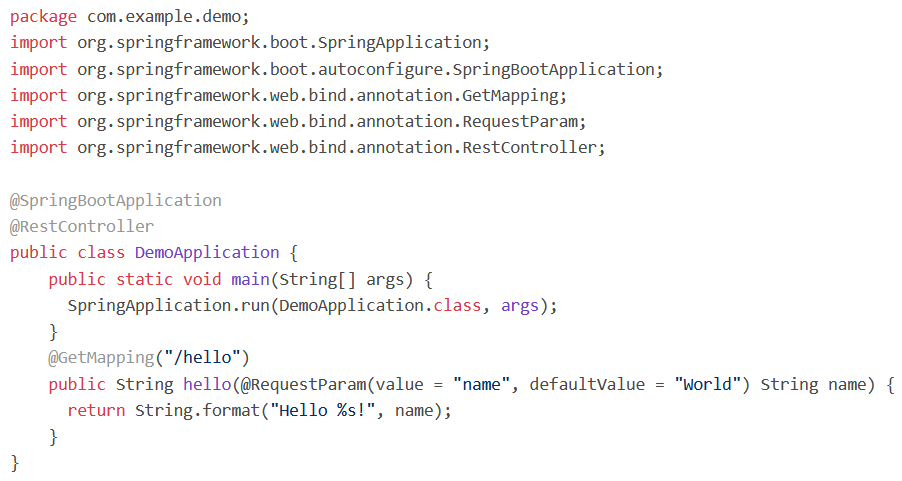
\includegraphics[width=0.2\textwidth]{images/springboot/exampleJavaSpringBootProgram.png}
    \caption{Przykładowy program java napisany z wykorzystaniem frameworku Springboot\cite{springJavaExampleProgram}}
    \label{fig:enter-label}
\end{figure}

Powyższy program składa się z głównej klasy aplikacji z adnotacją @SpringBootApplication, która wskazuje klasę konfiguracyjną, która deklaruje jedną lub więcej metod @Bean, a także uruchamia automatyczną konfigurację i skanowanie komponentów. Klasa DemoApplication zawiera główną metodę, która jest punktem wejścia aplikacji. Metoda SpringApplication.run uruchamia cały framework Spring.
Dodatkowo klasa jest opatrzona adnotacją @RestController, wskazującą, że jest to kontroler sieciowy, w którym każda metoda zwraca obiekt domeny zamiast widoku. Metoda hello jest mapowana do punktu końcowego /hello przy użyciu adnotacji @GetMapping, co pozwala jej obsługiwać żądania HTTP GET. Metoda ta przyjmuje nazwę parametru żądania z domyślną wartością „World” i zwraca wiadomość powitalną.

\section{Netflix Eureka}

\begin{figure}[!htbp]
    \centering
    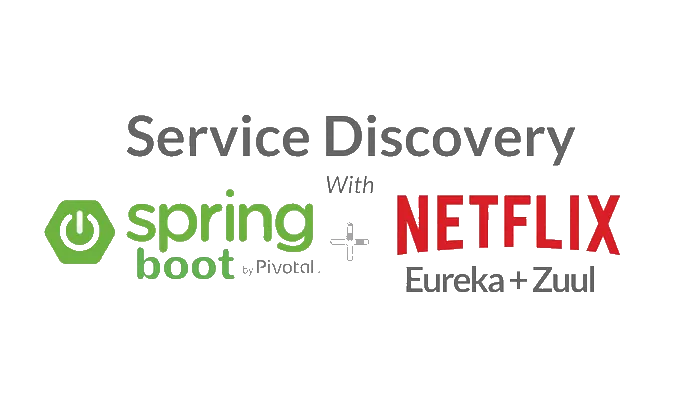
\includegraphics[width=0.2\textwidth]{images/netflixEureka/netflixEurekaLogo.png}
    \caption{Spring Cloud Netflix\cite{netflixEurekaMedium}}
    \label{fig:enter-label}
\end{figure}

Odnajdywanie usług jest jednym z kluczowych założeń architektury opartej na mikrousługach. Próba ręcznego konfigurowania każdego klienta lub jakiejś formy usługodawcy może być trudna do wykonania i ulotna ze względu na zmieniające się adresy w sieci komputerowej. Usługa odkrywania (\english{Service Discovery}) jest to proces automatycznego odnajdywania i wykrywania usług i urządzeń w sieci. Serwer Eureka to usługa oparta na \akronim{REST} (\english{Representational State Transfer}), która jest wykorzystywana głównie w chmurze Amazon \akronim{AWS} (\english{Amazon Web Services}) do lokalizowania usług w celu równoważenia obciążenia i przełączania awaryjnego serwerów. Eureka jest również dostarczana z komponentem klienckim opartym na Javie, Eureka Client, który znacznie ułatwia komunikacje z usługą\cite{netflixEurekaArticleWang}\cite{netflixEurekaGithub}\cite{springEureka}\cite{netflixEurekaManual}.

\begin{figure}[!htbp]
    \centering
    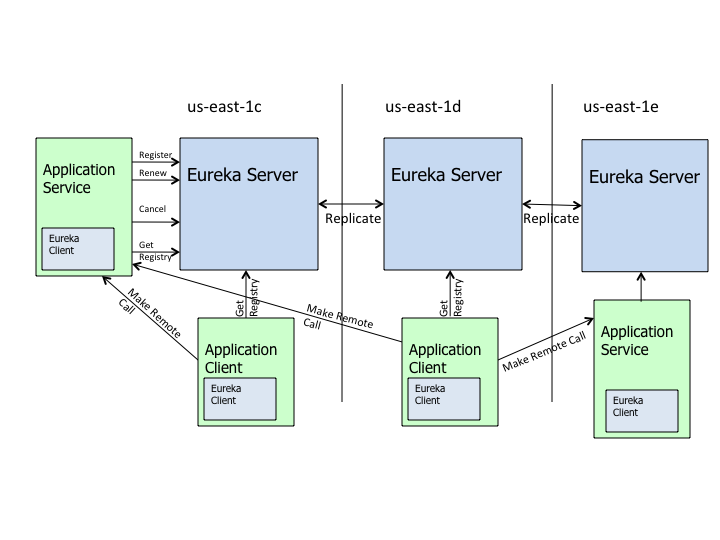
\includegraphics[width=\textwidth, trim={0 4cm 0 0}]{images/netflixEureka/eureka_architecture.png}
    \caption{przykładowa architektura klastra usług Eureka w Netflixie\cite{netflixEurekaGithub}}
    \label{fig:enter-label}
\end{figure}

Powyższa architektura przedstawia sposób, w jaki Eureka jest wdrażana w Netflixie i jest to typowy sposób jej uruchamiania. Na każdy region przypada jedna usługa (bądź też klaster usług) Eureka, w którym rejestrują się instancje z tego regionu, w którym jest uruchomiona. Usługi rejestrują się w serwerze Eureka, a następnie co 30 sekund wysyłają wiadomość hearbeat (\english{heartbeats}), aby odnowić swoje dzierżawy. Jeżeli usługa nie może odnowić dzierżawy kilka razy, jest ona usuwana z rejestru serwera w ciągu około 90 sekund. Informacje o rejestracji i odnowieniach są replikowane na wszystkich węzłów Eureka w klastrze. Klienci z dowolnej strefy mogą wyszukiwać informacje w rejestrze, aby zlokalizować swoje usługi (które mogą znajdować się w innej strefie niż klient) następnie po otrzymaniu informacji o szukanej instancji, klient wykonuje połączenie do usługi\cite{netflixEurekaArticleWang}\cite{netflixEurekaGithub}\cite{springEureka}\cite{netflixEurekaManual}.

\section{Docker}

\begin{figure}[!htbp]
    \centering
    
\includegraphics[width=0.2\textwidth]{images/Docker_logo.png}
    \caption{Logo marki Docker \cite{DockerMedia}}
    \label{fig:enter-label}
\end{figure}

W przeszłości aplikacje były zazwyczaj wdrażane na serwerach fizycznych lub maszynach wirtualnych. Przed wdrożeniem aplikacji należy skonfigurować niezbędną infrastrukturę. Obejmowało to instancję systemu operacyjnego, wszelkich zależności wymaganych przez aplikację i skonfigurowanie wszystkiego by ze sobą współpracowało w prawidłowy sposób. Było to czasochłonne i skomplikowane, zwłaszcza gdy próbowało się odtworzyć dokładnie to środowisko, dla którego aplikacja została stworzona.
Maszyny wirtualne stanowią pod tym względem znaczącą przewagę nad serwerami fizycznymi. Umożliwiają one programistom oddzielenie tworzonego oprogramowania od bazowego systemu. Dodatkowo, oferują one deweloperom łatwo dostępne środowisko, które mogli wykorzystywać do rozwoju i testowania, oddzielone od głównego systemu operacyjnego. Jednak maszyny wirtualne także posiadają swój własny zestaw wyzwań\cite{dockerContenerizationKeyAndUseCases}. 

Jednym z głównych problemów jest to, że wymagają one pełnej kopii systemu operacyjnego. Oznacza to, że są one stosunkowo duże i zajmują dużo zasobów. Z tego powodu uruchamianie wielu maszyn wirtualnych na tym samym serwerze fizycznym jest stosunkowo kosztowne. Kosztowne z dwóch perspektyw. Nie tylko uruchomienie setek maszyn wirtualnych kosztuje znaczną ilość pieniędzy, ale także wymaga dużej ilości zasobów, takich jak rdzenie procesora, pamięć \acronym{RAM} (\english{Random Access Memory}) i przestrzeń dyskowa. Co więcej, trudno jest skalować aplikacje w poziomie, co oznacza konieczność  dodania większej liczby replik aplikacji w celu obsłużenia zwiększonego ruchu, liczby użytkowników, czy obciążenia pracy danej repliki \cite{dockerContenerizationKeyAndUseCases}.

Konteneryzacja oferuje natomiast szereg korzyści, które pozwalają sprostać tym wyzwaniom. Dzięki konteneryzacji, deweloperzy mogą spakować swoje aplikacje i ich zależności w jednym kontenerze. Kontener ten może natomiast dostarczyć i wdrożyć na dowolnej platformie, która je obsługuje. Ułatwia to wdrożenie i uruchamianie aplikacji w rożnych środowiskach. Konteneryzacja oferuje spójne i niezawodne działanie aplikacji na różnych platformach, niezależnie od tego czy jest to serwer fizyczny, maszyna wirtualna w chmurze, czy też system operacyjny Windows lub Linux\cite{dockerContenerizationKeyAndUseCases}\cite{dockerOverview}. 

Dodatkowymi atutami konteneryzacji są:

\begin{itemize}
    \item \textbf{Przenaszalność}: Konteneryzowanie aplikacji może łatwo przenieść między różnymi środowiskami. Na przykład, można je łatwo przenieść z laptopa dewelopera do środowiska przejściowego lub produkcyjnego. Nie trzeba martwić się o różne konfiguracje między laptopem a serwerem, na którym zostanie wdrożony kontener\cite{dockerContenerizationKeyAndUseCases}\cite{dockerOverview}.
    
    \item \textbf{Izolacja}: Kontenery zapewniają warstwę izolacji między aplikacją a systemem hosta. Jest to coś w rodzaju bariery ochronnej, która pomaga zapobiegać konfliktom między różnymi aplikacjami lub zależnościami. Każdy kontener działa w swoim własnym, odizolowanym środowisku. Oznacza to, że jest mniej prawdopodobne, że wpłyną na niego inne aplikacje lub procesy działające na tej samej maszynie hosta. W związku z tym znacznie trudniej jest aplikacjom w kontenerach negatywnie wpływać na siebie nawzajem lub na system hosta. Pliki w systemie hosta i w innych kontenerach pozostaną nienaruszone, ponieważ aplikacja nie może uzyskać dostępu do plików spoza własnego środowiska\cite{dockerContenerizationKeyAndUseCases}\cite{dockerOverview}.

    \item \textbf{Wydajność zasobów}: Kontenery umożliwiają uruchamianie wielu odizolowanych aplikacji w tym samym systemie hosta. Nie trzeba przydzielać zasobów do każdej z nich z osobna (jak ma to miejsce w przypadku maszyn wirtualnych). Skutkuje to znacznym zmniejszeniem wykorzystania zasobów i kosztów. Ta zaleta jest szczególnie korzystna w środowiskach chmurowych, gdzie opłaty są często oparte na wykorzystaniu zasobów\cite{dockerContenerizationKeyAndUseCases}\cite{dockerOverview}.

    \item \textbf{Łatwe pakowanie, dostarczanie i wdrażanie}: Dla dewelopera spakowanie aplikacji do obrazu kontenera jest prostym procesem. Następnie deweloper może przesłać zbudowany obraz do rejestru kontenerów, który działa jako scentralizowany serwer do dystrybucji obrazu innym osobom. W ten sposób inne osoby mogą w prosty sposób pobrać zbudowany obraz na swoje urządzenie i go uruchomić\cite{dockerContenerizationKeyAndUseCases}\cite{dockerOverview}.
\end{itemize}

W 2013 roku pojawił się Docker, który sprawił że korzystanie z kontenerów stało się niezwykle proste. Dzięki Dockerowi można było tworzyć obrazy, przesyłać je do repozytorium, uruchamiać kontenery, łączyć je w sieci i wykonywać wiele innych zadań związanych z kontenerami. Oznacza to, że wystarczy użyć tylko jednego narzędzia aby obsłużyć wszystkie potrzeby związane z kontenerami. W rezultacie kontenery stały się głównym nurtem i zyskały ogromną popularność\cite{dockerContenerizationKeyAndUseCases}\cite{dockerOverview}.

\subsubsection{Docker Compose}

Docker Compose to narzędzie do definiowania i uruchamiania aplikacji wielokontenerowych. Jest to klucz do odblokowania usprawnionego i wydajnego środowiska programowania i wdrażania.
Compose upraszcza kontrolę nad całym stosem aplikacji, ułatwiając zarządzanie usługami, sieciami i wolumenami w jednym, zrozumiałym pliku konfiguracyjnym \akronim{YAML} (\english{YAML Ain’t Markup Language}). Następnie za pomocą jednego polecenia można utworzyć i uruchomić wszystkie usługi z pliku konfiguracyjnego. Compose działa we wszystkich środowiskach: produkcyjnym, przejściowym, deweloperskim, testowym, a także w przepływach pracy \akronim{CI} (\english{Continuous Integration})\cite{dockerComposeAStudyMultiContainerSystem}\cite{dockerComposeOverview}\cite{dockerComposePaterns}.

Posiada również polecenia do zarządzania całym cyklem życia aplikacji: 
\begin{itemize}
    \item Uruchamianie, zatrzymywanie i przebudowywanie stosu usług
    \item Wyświetlenie stanu uruchomionych aplikacji
    \item Przesyłanie strumieniowe danych wyjściowych dziennika uruchomionych usług
    \item Uruchamianie jednorazowego polecenia w określonym kontenerze
\end{itemize}

\section{Elasticsearch}

\begin{figure}[!htbp]
    \centering
    \includesvg[width=0.1\textwidth]{images/ELK-Stack/logo-elasticsearch-32-color.svg}
    \caption{Logo Elasticsearch \cite{elasticSearchManualDataIn}}
    \label{fig:enter-label}
\end{figure}

Elasticsearch to rozproszony magazyn dokumentów. Zamiast przechowywać informacje w postaci encji, Elasticsearch przechowuje złożone struktury danych, które zostały serializowane jako dokumenty \akronim{JSON} (\english{JavaScript Object Notation}). W przypadku posiadania wielu węzłów Elasticsearch w klastrze, przechowywane dokumenty są dystrybuowane w całym klastrze i można uzyskać do nich natychmiastowy dostęp z dowolnego węzła\cite{elasticSearchManualDataIn}. 

Elasticsearch jest zbudowany tak, aby był zawsze dostępny i skalował się zgodnie z wymaganiami systemu w którym pracuje. Osiąga to dzięki swojej rozproszonej naturze. Dodając węzły do klastra zwiększając jego pojemność następnie Elasticsearch automatycznie rozdzieli dane i obciążenie na wszystkie dostępne węzły. Nie ma potrzeby przebudowywania aplikacji, Elasticsearch sam zrównoważy klastry wielowęzłowe, aby zapewnić wysoką dostępność.

Gdy dokument jest przechowywany w systemie, jest indeksowany i w pełni przeszukiwalny. Elasticsearch wykorzystuje strukturę danych zwaną odwróconym indeksem, który obsługuje bardzo szybkie wyszukiwanie pełnotekstowe. Odwrócony indeks wyszczególnia każde unikalne słowo, które pojawia się w dowolnym dokumencie i identyfikuje wszystkie dokumenty, w których każde słowo występuje\cite{elasticSearchManualDataIn}.  

Indeks można traktować jako zoptymalizowaną kolekcję dokumentów, a każdy dokument jest zbiorem pól, które są parami klucz--wartość zawierającymi dane. Domyślnie Elasticsearch indeksuje wszystkie dane w każdym polu, a każde indeksowane pole ma dedykowaną, zoptymalizowaną strukturę danych.
Na przykład pola tekstowe są przechowywane w indeksach odwróconych, a pola numeryczne i geograficzne są przechowywane w drzewach \akronim{BKD}. Zdolność do korzystania ze struktur danych dla poszczególnych typów pól do gromadzenia i zwracania wyników wyszukiwania sprawia, że Elasticsearch jest tak szybki\cite{elasticSearchManualDataIn}.

Elasticsearch ma również możliwość bycia bez schematu, co oznacza że dokumenty mogą być indeksowane bez wyraźnego określenia sposobu obsługi każdego z pól, które mogą wystąpić w dokumencie. Gdy dynamiczne mapowanie jest włączone, Elasticsearch automatycznie wykrywa i dodaje nowa pola do indeksu. To domyślne zachowanie ułatwia indeksowanie i eksplorację danych, w momencie indeksowania, Elasticsearch wykrywa i mapuje wartości logiczne, zmiennoprzecinkowe, całkowite, daty i ciągi znaków na odpowiednie typy danych\cite{elasticSearchManualDataIn}. 

Ostatecznie jednak użytkownik wie więcej o swoich danych i sposobie ich wykorzystania niż Elasticsearch. Użytkownik może zdefiniować reguły kontrolujące dynamiczne mapowanie i jawnie zdefiniować konwersję, aby przejąć pełną kontrolę nad sposobem przechowywania i indeksowania pól\cite{elasticSearchManualDataIn}.

Definiowanie własnych mapowań umożliwia:

\begin{itemize}
    \item Rozróżnianie pełnotekstowych pól łańcuchowych i pól łańcuchowych z dokładną wartością.
    \item Przeprowadzanie analizy tekstu specyficznej dla języka
    Optymalizację pól pod kątem częściowego dopasowywania
    \item Używanie niestandardowych formatów daty
    \item Używanie typów danych, takich jak \verb|geo_point| i \verb|geo_shape|, których nie można wykryć automatycznie.
\end{itemize}

Często przydatne jest indeksowanie tego samego pola na różne sposoby w różnych celach. Na przykład, użytkownik może chcieć indeksować pole łańcuchowe zarówno jako pole tekstowe do wyszukiwania pełnotekstowego, oraz jako pole słów kluczowych do sortowania lub agregowania danych. Można też użyć więcej niż jednego analizatora języka do przetworzenia zawartości pola łańcuchowego zawierającego dane wejściowe użytkownika\cite{elasticSearchManualDataIn}.

\section{Logstash}

\begin{figure}[!htbp]
    \centering
    \includesvg[width=0.1\textwidth]{images/ELK-Stack/logo-logstash-32-color.svg}
    \caption{Logstash logo\cite{logstashMain}}
    \label{fig:enter-label}
\end{figure}

Logstash to silnik gromadzenia danych typu otwarto źródłowego (\english{Open source}) z możliwością potokowania w czasie rzeczywistym. Logstash może dynamicznie ujednolicić dane z różnych śródeł i normalizować je do wybranych miejsc docelowych. Oczyszcza i demokratyzuje wszystkie dane dla różnorodnych zaawansowanych zastosować analiztycznych i wizualizacyjnych\cite{logstashManualIntroduction}.

Logstash pierwotnie napędzał innowacje w zakresie gromadzenia logów, jego możliwości wykraczają dlatego poza ten przypadek użycia. Każdy rodzaj zdarzenia można wzbogacić i przekształcić za pomocą szerokiej gamy wtyczek wejściowych, filtrujących i wyjściowych, a wiele natywnych kodeków dodatkowo upraszcza proces pozyskiwania danych. Logstash przyspiesza pozyskiwanie informacji poprzez wykorzystanie większej ilości i różnorodności danych\cite{logstashManualIntroduction}.

Potok przetwarzania zdarzeń Logstash składa się z trzech etapów:

\begin{figure}[!htbp]
    \centering
    \includesvg[width=0.15\textwidth]{schemas/logstashPipeline.drawio.svg}
    \caption{Przetwarzanie zdarzeń w logstash}
    \label{fig:enter-label}
\end{figure}

Wejścia generują zdarzenia, następnie są one filtrowane aby ostatecznie wyjścia wysłały je do miejsca docelowego. Wejścia i wyjścia obsługują kodeki, które umożliwiają kodowanie lub dekodowanie danych wchodzących lub wychodzących z potoku bez konieczności  stosowania oddzielnego filtra\cite{logstashManualHowItWorks}. 

\subsubsection{Wejścia}

Wejścia służą do pobierania danych do Logstash. Niektóre z najczęściej używanych wejść to:

\begin{itemize}
    \item file: odczyt z pliku w systemie plików, podobnie jak w polecenie w UNIX \termdef{tail -0F}\cite{logstashManualHowItWorks}.
    \item syslog: nasłuchuje na porcie 514 i analizuje je zgodnie z formatem RFC3164\cite{rfc3164}\cite{logstashManualHowItWorks}.
    \item redis: oczytuje z serwera redis, używając zarówno kawałków oraz list. Redis jest często używany jako "broker" w scentralizowanym systemie. Logstash, który kolejkuje zdarzenia od zdalnych nadawców\cite{logstashManualHowItWorks}.
    \item beats: przetwarza zdarzenia wysłane przez Beats\cite{logstashManualHowItWorks}.
\end{itemize}

\subsubsection{Filtry}

Filtry są pośrednimi urządzeniami przetwarzającymi w potoku. Filtry można łączyć z instrukcjami warunkowymi w ceu wykonania akcji na zdarzeniu, jeśli spełnia ono określone kryteria. Niektóre przydatne filtry obejmują: 

\begin{itemize}
    \item \textbf{grok}: parsuje i strumieniuje dowolny tekst. Grok jest obecnie najlepszym sposobem w Logstash na analizowanie nieustrukturyzowanych danych dziennika w celu przetworzenia danych w formę nadającą się do zapytań\cite{logstashManualHowItWorks}. 
    \item \textbf{mutate}: wykonuje ogólne transformacje na polach zdarzeń. Można edytować nazwy, usuwać, zastępować i modyfikować pola w zdarzeniach.
    \item \textbf{drop}: pozwala na całkowicie odrzucenie zdarzenia\cite{logstashManualHowItWorks}.
    \item \textbf{clone}: tworzy kopię zapasową zdarzenia, ewentualnie dodając lub usuwając pola\cite{logstashManualHowItWorks}.
    \item \textbf{geoip}: dodawanie informacji o położeniu geograficznym adresów IP\cite{logstashManualHowItWorks}.
\end{itemize}

\subsubsection{Wyjścia}

Wyjścia są ostatnią fazą potoku Logstash. Zdarzenie może przechodzić przez wiele wyjść, ale po zakończeniu przetwarzania wszystkich danych wyjściowych zdarzenie kończy swoje wykonanie\cite{logstashManualHowItWorks}.
Niektóre często używane wyjścia obejmują:

\begin{itemize}
    \item \textbf{elasticsearch}: wysyła dane zdarzeń do Elasticsearch\cite{logstashManualHowItWorks}.
    \item \textbf{file}: zapisywanie danych zdarzeń do pliku na dysku\cite{logstashManualHowItWorks}.
    \item \textbf{graphite}: wysyła dane do zdarzeń do graphite, popularnego otwarto źródłowego narzędzia do przechowywania i tworzenia wykresów metryk\cite{logstashManualHowItWorks}.
\end{itemize}

\subsubsection{Kodeki}

Kodeki to filtry strumieniowe, które mogą działać jako część wejścia lub wyjścia. Kodeki umożliwiają łatwe oddzielenie transportu wiadomości od procesu serializacji. Do najpopularniejszych kodeków należą:

\begin{itemize}
    \item \textbf{json}: koduje lub dekoduje dane w formacie JSON\cite{logstashManualHowItWorks}.
    \item \textbf{multiline}: łączy wielowierszowe zdarzenia tekstowe, takie jak wyjątki w javia i komunikaty zrzutem stosu (\english{Stack trace}) w jedno zdarzenie\cite{logstashManualHowItWorks}.
\end{itemize}

\section{Metricbeat}


\begin{figure}[!htbp]
    \centering
    \includesvg[width=0.1\textwidth]{images/ELK-Stack/icon-metricbeat-32-color.svg}
    \caption{Logo Metricbeat\cite{metricbeatLogo}}
    \label{fig:enter-label}
\end{figure}

Metricbeat to program wykorzystywany do okresowego zbierania metryk z systemu operacyjnego i usług działających na serwerze. Metricbeat pobiera zebrane metryki i statystyki a następnie wysyła je do okreslonych przez użytkownika punktów docelowych, takich jak Elasticsearch, Logstash, Redis lub Kafka\cite{metricbeatOverview}.


\section{Kibana}

\begin{figure}[!htbp]
    \centering
    \includesvg[width=0.1\textwidth]{images/ELK-Stack/logo-kibana-32-color.svg}
    \caption{Logo Kibana\cite{kibanaLogo}}
    \label{fig:enter-label}
\end{figure}

Kibana jest to narzędzie do wizualizacji i eksploracji danych wykorzystywane do analizy dokumentów, przechowywanych w stosie oprogramowania Elastic. Kibana umożliwia nadanie kształtu danym oraz poruszanie się po stosie oprogramowania Elastic\cite{kibanaOverview}. 

Kibana między innymi zapewnia następujące funkcjonalności:

\begin{itemize}
    \item \textbf{Wyszukiwanie, obserwowanie i chronienie danych}: Odkrywanie dokumentów,  analizowanie dzienników oraz znajdowanie luk w zabezpieczeniach\cite{kibanaOverview}.
    \item \textbf{Analiza danych}: Wyszukiwanie zależności, wizualizacja danych na grafach, diagramach, mapach oraz tworzenie, pulpitów nawigacyjnych\cite{kibanaOverview}.
    \item \textbf{Monitoring}: Kibana zapewnia możliwość monitorowania całego klastra oprogramowania Elastic oraz kontrolowania dostępu użytkowników do poszczególnych funkcjonalności\cite{kibanaOverview}.
\end{itemize}

\section{Logstash Logback Encoder}

Logstash Logback Encoder to biblioteka zaprojektowana w celu ułatwienia rejestrowania dzienników aplikacji w formacie JSON przy użyciu biblioteki Logback. Koder ten umożliwia ustrukturyzowanie przechowywanie zdarzeń w formacie JSON, ułatwiając analizowanie dzienników przy wykorzystaniu takich narzędzi jak Logstash i Elasticsearch\cite{logstashLogbackEncoderOverview}. 

Kluczowe cechy:

\begin{itemize}
    \item \textbf{Kodowanie JSON}: Podstawową funkcją tego kodera jest kodowanie zdarzeń Logback do formatu JSON\cite{logstashLogbackEncoderOverview}.
    \item \textbf{Konfigurowalny wygląd}: Biblioteka pozwala na dostosowanie układów logów, umożliwiając użytkownikom zdefiniowanie własnej struktury zdarzeń\cite{logstashLogbackEncoderOverview}.
    \item \textbf{Zaawansowane dodatki}: Dodatkowe appendery, takie jak LogstashTcpSocketAppender i AsyncDisruptorAppender, które ułatwiają wysyłanie logów przez sieć lub ich asynchroniczną obsługę\cite{logstashLogbackEncoderOverview}.
    \item \textbf{Wsparcie dla filtrów Logback}: Biblioteka obsługuje filtry Logback, umożliwiając warunkowe logowanie w oparciu o niestandardowe kryteria\cite{logstashLogbackEncoderOverview}.
    \item \textbf{Maskowanie i zmiana}: Wrażliwe informacje w dziennikach mogą być maskowane lub zmieniane w celu zapewnienia zgodności z przepisami dotyczącymi prywatności danych\cite{logstashLogbackEncoderOverview}.
\end{itemize}

Biblioteka jest szczególnie wykorzystywana w systemach rozproszonych do centralizacji dzienników aplikacyjnych z wielu źródeł i usprawniania ich analizy za pomocą narzędzi takich jak stos \akronim{ELK} (Elasticsearch, Logstash, Kibana)\cite{logstashLogbackEncoderOverview}.

Aby zintegrować Logstash Logback Encoder z projektem Java, należy uwzględnić go jako zależność w konfiguracji kompilacji w pliku konfiugracyjnym, dodatkowo należy skonfigurować plik \textit{logback-spring.xml}, tak aby biblioteka korzystała z prawidłowych appenderów\cite{logstashLogbackEncoderOverview}.